\documentclass[12pt]{article}

\usepackage{graphicx}
\usepackage{float}
\renewcommand\refname{Bibliografia} 
	
\begin{document}


\begin{titlepage}
  \begin{center}
    
\includegraphics[scale=0.1]{img/logo-unipd.png}\\

    \vspace{0.8cm}
    \textsc{\LARGE Universit\`{a} degli Studi di Padova}\\
    \vspace{0.45cm}
    \textsc{\large Dipartimento di Ingegneria Industriale}\\
    \vspace{0.4cm}
    \textsc{\large Corso di Laurea in}\\
    \textsc{\large Ingegneria Aerospaziale}\\
    \vspace{1.2cm}
    \textsc{\large Tesi di Laurea}\\
    \vfill
    % Title
    { \LARGE \bfseries Raccolta e analisi dei dati di volo per un velivolo a controllo remoto
    }\\
    \vfill
    \textit{\large Relatore:} \hfill \textit{\large Laureando:}\\
    \textsc{\large Prof. Francesco Picano} \hfill \textsc{Emanuele Cason}\\
    \hfill \textsc{1219779}\\

    \vfill
    {\large Anno Accademico 2022/2023}
  \end{center}
\end{titlepage}

\section*{Introduzione}
Nell'ambito del progetto LiftUp del Dipartimento di Ingegneria Industriale, per la partecipazione all'Air Cargo Challenge 2022, è stato progettato e costruito un velivolo a controllo remoto, candidato poi dal nostro team alla competizione.
Tutto il processo di progettazione e realizzazione del drone, di seguito denominato UAS (Unmanned Aerial System), secondo la nomenclatura adottata dal legislatore europeo, si è basato sul regolamento di gara, e in particolare sui requisiti di sistema e sui criteri di attribuzione del punteggio. Di tali criteri, la porzione più rilevante è stata dedicata dalla giuria alle prestazioni in volo dell'aeromobile. Ne è nata la necessità di integrare un sistema di registrazione e trasmissione dei dati di volo dei sensori, al fine di valutare le prestazioni durante il collaudo, individuare le migliori condizioni di manovra e prevedere i punteggi conseguenti alle singole esercitazioni di preparazione svolte nei mesi precedenti alla gara.

\section*{Sistema di telemetria - versione 1}
La scelta di implementare una prima versione di sistema di telemetria è stata conseguente alla necessità immediata di ottenere i dati fondamentali già dalle prime uscite in campo di volo. Si è quindi selezionato un modulo di logging dei dati (SM-Modellbau GPS-Logger 3), integrante un ricevitore GNSS (Global Navigation Satellite System), accelerometro a tre assi e barometro, con registrazione su scheda microSD. La scelta del componente è derivata da vari fattori considerati: i valori di risoluzione e velocità di aggiornamento dei dati relativamente alti, la compatibilità con i sistemi a bordo dell'aeromodello e di radiocontrollo, la consistenza dei dati con quelli che sarebbero stati raccolti in competizione (dove da regolamento, la giuria utilizza lo stesso modulo per calcolare i punteggi di gara), e non ultimo il basso costo.

\subsection*{Implementazione del modulo}
Da un punto di vista di compatibilità con il sistema aeromodello, il modulo utilizzato, permette di essere alimentato con tensioni all'interno del range tra 3.6 V e 8.5 V, dispone di un ingresso PWM per leggere il segnale di un canale del modulo ricevente ed è compatibile con il protocollo Smart Port che utilizza il radiocomando, permettendo di trasmettere a quest'ultimo i dati di telemetria, che a seguito della programmazione necessaria li rende visibili nel suo display. Per minimizzare l'effetto radio schermante della fibra di carbonio di cui è largamente composto il velivolo, si è posizionato il ricevitore in un'apposita baia, nella zona superiore della fusoliera. Di conseguenza, il modulo è stato implementato secondo lo schema seguente:

\begin{figure}[H]
	\centering
	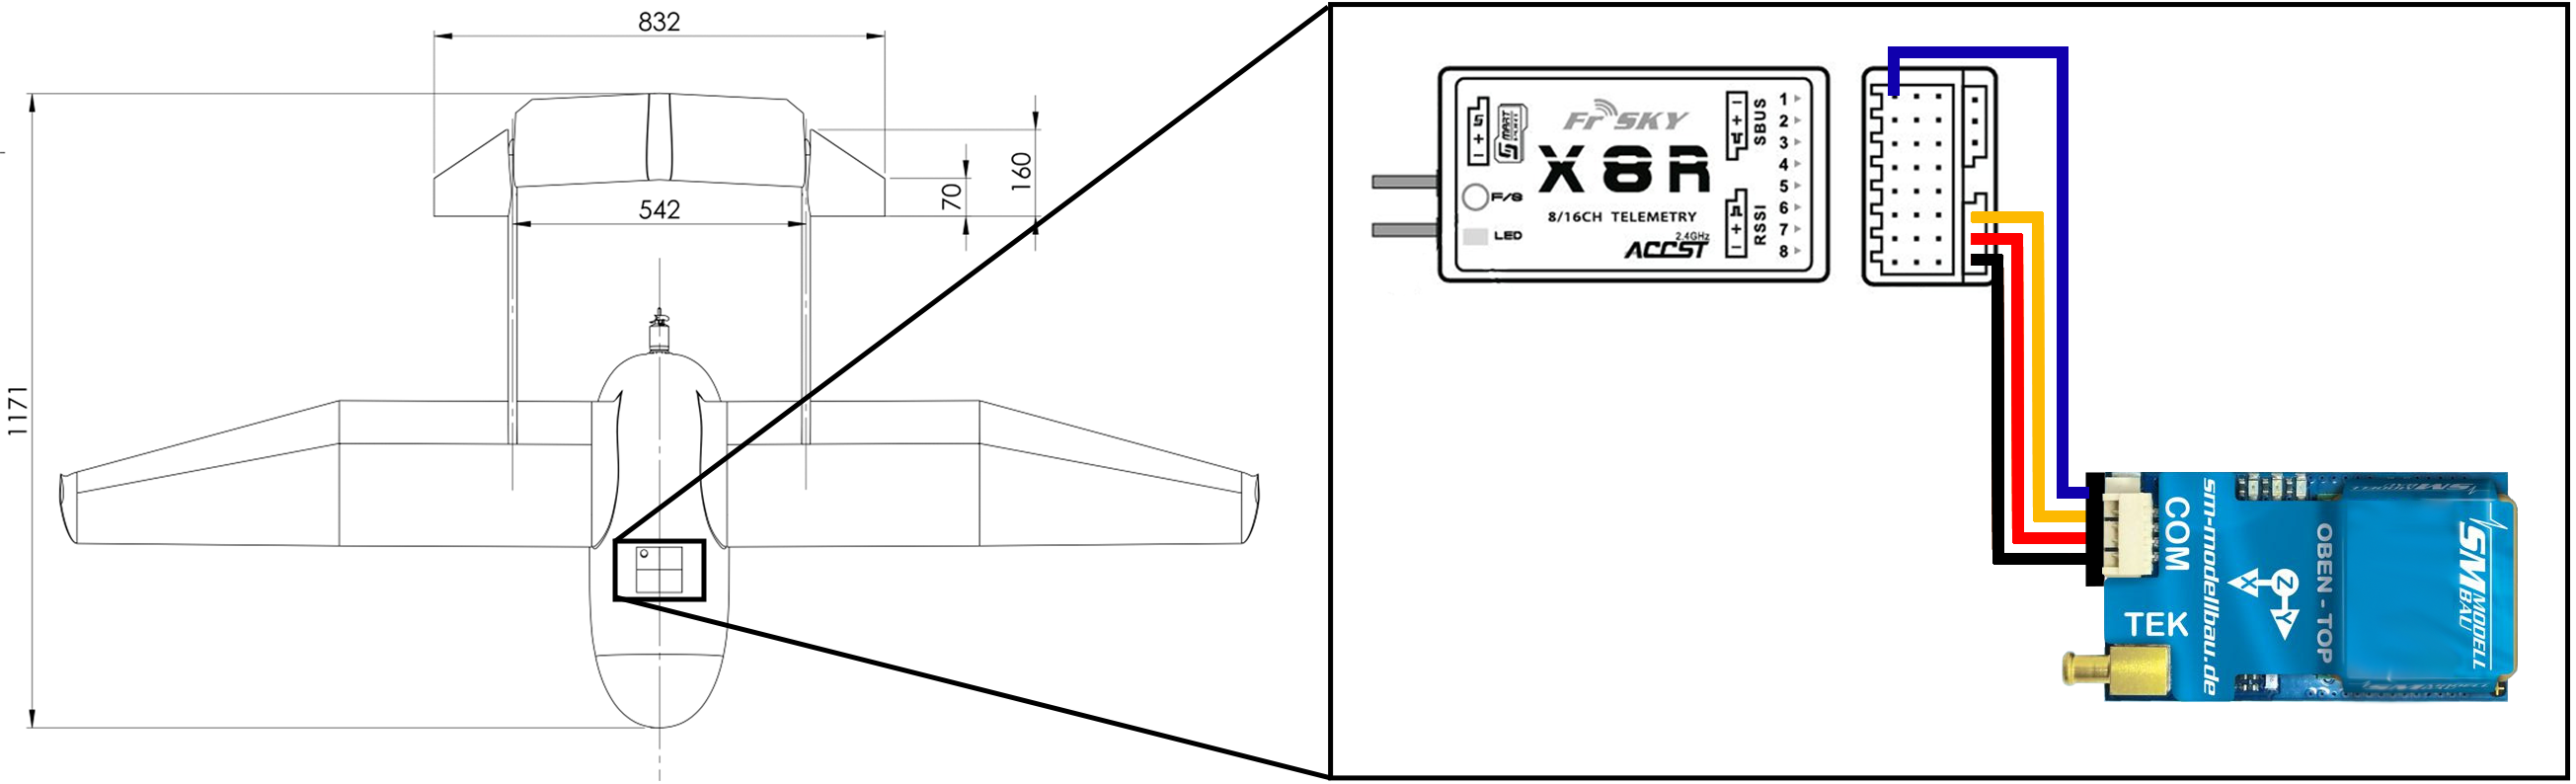
\includegraphics[width=14cm]{img/Schema-v1}
\end{figure}

\subsection*{Criteri di attribuzione del punteggio di volo}
I tre fattori principali per l'attribuzione del punteggio del singolo volo, come da regolamento \textsuperscript{\cite{regulation}}, sono stati:
\begin{itemize}
\item \textbf{Payload} trasportato durante il volo, misurato in termini di massa.
\item \textbf{Altitudine} raggiunta a 60 secondi del tempo di volo.
\item \textbf{Distanza} coperta durante i primi 180 secondi del tempo di volo.
\end{itemize}
Dove l'inizio della misura del tempo di volo è stato definito in corrispondenza del raggiungimento di 5 km/h di velocità rispetto al suolo (misurata dal modulo GPS), durante la fase di decollo.

\newpage
\bibliography{refs}
\bibliographystyle{plain}


\end{document}